\documentclass[11pt, oneside]{article}   	% use "amsart" instead of "article" for AMSLaTeX format

%
%	TikZ
%
\usepackage{tikz}
\usetikzlibrary{calc,patterns,angles,quotes,shapes,math,decorations,through,intersections,lindenmayersystems,backgrounds}    
\usepackage{tkz-euclide}
\usepackage{pgfplots}
%
%
%
\usepackage[margin=1.0in]{geometry}                                     % adjust margins
\geometry{letterpaper}                                                  % ... or a4paper or a5paper or ... 
% \usepackage{url}                                                        % need this to use URLs in bibtex
% \usepackage{setspace}                                                   % need this for \setstrech{...}
% \usepackage{scrextend}                                                  % need this for addmargin
% \usepackage[export]{adjustbox}                                          % need this to get frame for includegraphics
% \usepackage{bigints}                                                    % bigger integral symbol
% \usepackage{amssymb}
% \usepackage{mathrsfs}
% \usepackage{hyperref}
% \usepackage{url}
% \usepackage{subcaption}
% \usepackage{authblk}
% \usepackage{amsmath}
% \usepackage{mathtools}
% \usepackage{graphicx}
% \usepackage[export]{adjustbox}
% \usepackage{hyperref}
% \usepackage{alltt}
% \usepackage{color}
% \usepackage[utf8]{inputenc}
% \usepackage[english]{babel}
\usepackage{float}
\usepackage{bigints}
\usepackage{braket}
\usepackage{siunitx}
\usepackage{relsize}
\usepackage{framed}


%
% compatability
%
\pgfplotsset{compat=1.17} 

\newcommand*{\Scale}[2][4]{\scalebox{#1}{$#2$}}%



% \usepackage{circuitikz}
\usepackage[oldvoltagedirection]{circuitikz}


\begin{document}



\begin{figure}[H]
\centering
\begin{framed}
\begin{equation*}
\begin{array}{llll}
f(x)
&=& {\mathlarger{\mathlarger \sum\limits_{n=0}^{\infty}}} \dfrac{f^{(n)} (a)}{n!}(x-a)^n \\
[20pt]
&=& \dfrac{f^{(0)}(a)}{0!} (x-a)^0 + \dfrac{f^{(1)}(a)}{1!} (x-a)^1 + \dfrac{f^{(2)}(a)}{2!} (x-a)^2 + \dfrac{f^{(3)}(a)}{3!} (x-a)^3 + \cdots \\
[15pt]
&=& f(a) + f^{(1)}(a)(x-a) + \dfrac{f^{(2)}(a)}{2} (x-a)^2 + \dfrac{f^{(3)}(a)}{6} (x-a)^3 + \dfrac{f^{(4)}(a)}{24} (x-a)^4 + \cdots 
\end{array}
\end{equation*}
\end{framed}
\caption{Taylor Series for $f(x)$ centered at $a$}
\label{fig:taylor_series_centered_at_a}
\end{figure}

\bigskip
\bigskip

\begin{figure}[H]
   \centering
   \resizebox{0.65 \textwidth}{!} {																	% resize figure if you want
   \begin{circuitikz}[framed,line width=0.75pt]
       \draw[step=0.5,thin, black!30] (-1.50,-0.5) grid (5.50,3.0);
       \path (0,0) coordinate (ref_gnd);
       \draw (ref_gnd) -- (ref_gnd) to [american voltage source=\(V\)] ++(0,2)
 %           to [R=\(R\)] ++(3,0) 
            to [L=\(L\)] ++(3,0) 
            to [C=\(C\)] ++(0,-2)
            to []  (ref_gnd);
       \draw [draw=none] (0,0) -- ({3+3},0) node [midway,above] {$I$};								% draw current (I) and direction arrow
       \draw [black,thick, -latex] (2.50,-0.25) -- ({((3+3)/2) + 0.50},-0.25) node [midway,below] {};
       \draw [draw=none] (ref_gnd) -- ({3+3},2.90) node [midway,above] {$I$};						% draw current (I) and direction arrow
       \draw [black,thick, latex-] (2.50,2.250) -- (3.50,2.250) node [midway,above] {};
   \end{circuitikz}
  }																									% end \resizebox
\caption{Series LC Circuit}
\label{fig:series_lc_circuit}
\end{figure}


\begin{figure}[H]
   \centering
   \resizebox{0.65 \textwidth}{!} {																	% resize figure if you want
   \begin{circuitikz}[framed,line width=0.75pt]
       \draw[step=0.5,thin, black!30] (-1.50,-0.5) grid (7.50,3.0);
       \path (0,0) coordinate (ref_gnd);
       \draw (ref_gnd) -- (ref_gnd) to [american voltage source=\(V\)] ++(0,2)
            to [R=\(R\)] ++(3,0) 
            to [L=\(L\)] ++(3,0) 
            to [C=\(C\)] ++(0,-2)
            to []  (ref_gnd);
       \draw [draw=none] (0,0) -- ({3+3},0) node [midway,above] {$I$};								% draw current (I) and direction arrow
       \draw [black,thick, -latex] (2.50,-0.25) -- ({((3+3)/2) + 0.50},-0.25) node [midway,below] {};
       \draw [draw=none] (ref_gnd) -- ({3+3},2.90) node [midway,above] {$I$};						% draw current (I) and direction arrow
       \draw [black,thick, latex-] (2.50,2.250) -- (3.50,2.250) node [midway,above] {};
   \end{circuitikz}
  }																									% end \resizebox
\caption{Series RLC Circuit}
\label{fig:series_rlc_circuit}
\end{figure}




\begin{figure}[H]
  \centering
  \resizebox{0.45 \textwidth}{!} {																% resize figure if you want
    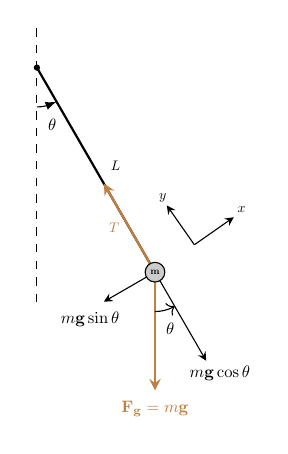
\begin{tikzpicture}
      \pgfmathsetmacro{\Gvec}{1.5}																% save length of g-vector and theta to macros
      \pgfmathsetmacro{\myAngle}{30}
      \pgfmathsetmacro{\Gcos}{\Gvec*cos(\myAngle)}												% calculate lengths of vector components
      \pgfmathsetmacro{\Gsin}{\Gvec*sin(\myAngle)}
%
%	make some coordinates
%
      \coordinate (centro) at (0,0);
      \draw[dashed] (0,0.5) -- ++(0,-3.5) node (mary) [black,below]{};
      \fill (centro) circle (0.04);
      \draw[thick] (centro) -- ++(270+\myAngle:3) coordinate (bob);
      \path (1.00,-1.25) node[] {$\Scale[0.5] {L}$}; 
      \draw [thick,brown,-stealth] (bob) -- ($(bob)!\Gcos cm!(centro)$) node[left,midway] {${\Scale[0.50] T}$};
%
%	draw the angle
%
     \pic [draw, -latex, "${\Scale[0.60]{\theta}}$", angle eccentricity=1.5] {angle = mary--centro--bob};
%
%	draw the rest of the pendulum
%
     \draw [-stealth] (bob) -- ($(bob)!-\Gcos cm!(centro)$)
       coordinate (gcos)
      node[midway,below, yshift=-0.5cm, xshift=0.50cm] {$\Scale[0.60] {m {\bf g} \cos\theta}$};
     \draw [-stealth] (bob) -- ($(bob)!\Gsin cm!90:(centro)$)
       coordinate (gsin)
     node[midway,below,yshift=-0.20cm, xshift=-0.50cm] {$\Scale[0.60] {m {\bf g} \sin \theta}$};
     \draw [thick,brown,-stealth] (bob) -- ++(0,-\Gvec)
       coordinate (g)
       node[below,brown] {$\Scale [0.60] {{\bf F_{g}} = m {\bf g}}$};
     \pic [draw, ->, "{$\Scale[0.60] {\theta}$}", angle eccentricity=1.5] {angle = g--bob--gcos};
     \filldraw [fill=black!20,draw=black] (bob) circle[radius=0.125];
     \path (bob) node[] {$\Scale[0.35] {\bf m}$};
%
%	draw the x-y coordinate system
%
     \draw [-stealth] (2.00,-2.25) -- (2.50,-1.90) node[xshift=0.10cm, yshift=0.10cm] {$\Scale[0.50] {x}$};
     \draw [-stealth] (2.00,-2.25) -- (1.65,-1.75) node[xshift=-0.05cm,yshift=0.10cm] {$\Scale[0.50] {y}$};
   \end{tikzpicture}
  }																							% end \resizebox
\caption{Free Body Diagram of a Simple Pendulum}
\label{fig:simple_pendulum}
\end{figure}



\end{document}
